\begin{figure*}[!t]
\centering
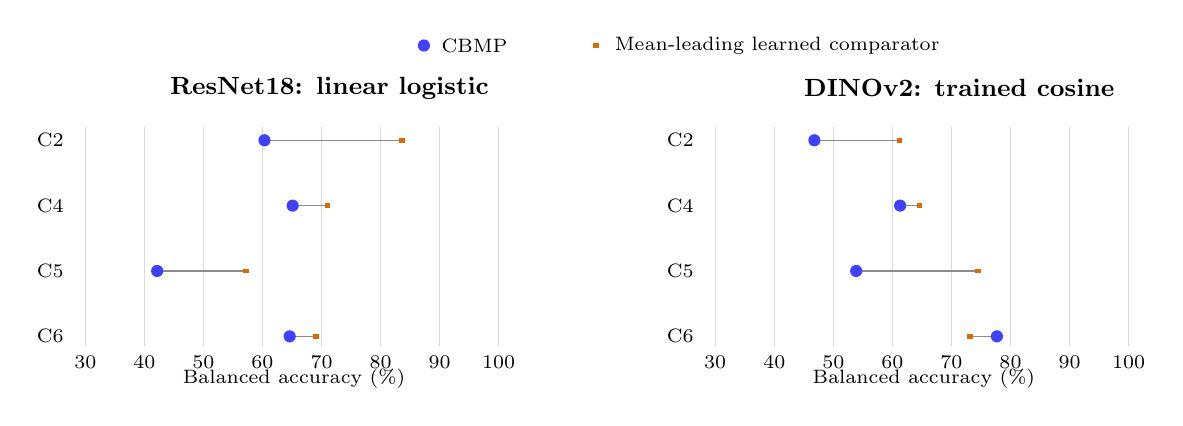
\begin{tikzpicture}[font=\scriptsize,y=.83cm]
\begin{scope}[xshift=0cm]
\node[font=\small\bfseries] at (3.1,3.8) {ResNet18: linear logistic};
\draw[black!15] (0.000000,-.15)--(0.000000,3.2);
\node[below] at (0.000000,-.15) {30};
\draw[black!15] (0.750000,-.15)--(0.750000,3.2);
\node[below] at (0.750000,-.15) {40};
\draw[black!15] (1.500000,-.15)--(1.500000,3.2);
\node[below] at (1.500000,-.15) {50};
\draw[black!15] (2.250000,-.15)--(2.250000,3.2);
\node[below] at (2.250000,-.15) {60};
\draw[black!15] (3.000000,-.15)--(3.000000,3.2);
\node[below] at (3.000000,-.15) {70};
\draw[black!15] (3.750000,-.15)--(3.750000,3.2);
\node[below] at (3.750000,-.15) {80};
\draw[black!15] (4.500000,-.15)--(4.500000,3.2);
\node[below] at (4.500000,-.15) {90};
\draw[black!15] (5.250000,-.15)--(5.250000,3.2);
\node[below] at (5.250000,-.15) {100};
\node[left] at (-.15,3) {C2};
\draw[black!45] (2.275416,3)--(4.018669,3);
\fill[blue!75] (2.275416,3) circle (2.2pt);
\fill[orange!85!black] (3.983669,2.965) rectangle (4.053669,3.035);
\node[left] at (-.15,2) {C4};
\draw[black!45] (2.632689,2)--(3.073368,2);
\fill[blue!75] (2.632689,2) circle (2.2pt);
\fill[orange!85!black] (3.038368,1.965) rectangle (3.108368,2.035);
\node[left] at (-.15,1) {C5};
\draw[black!45] (0.912446,1)--(2.037976,1);
\fill[blue!75] (0.912446,1) circle (2.2pt);
\fill[orange!85!black] (2.002976,0.965) rectangle (2.072976,1.035);
\node[left] at (-.15,0) {C6};
\draw[black!45] (2.595662,0)--(2.931159,0);
\fill[blue!75] (2.595662,0) circle (2.2pt);
\fill[orange!85!black] (2.896159,-0.035) rectangle (2.966159,0.035);
\node at (2.65,-.65) {Balanced accuracy (\%)};
\end{scope}
\begin{scope}[xshift=8cm]
\node[font=\small\bfseries] at (3.1,3.8) {DINOv2: trained cosine};
\draw[black!15] (0.000000,-.15)--(0.000000,3.2);
\node[below] at (0.000000,-.15) {30};
\draw[black!15] (0.750000,-.15)--(0.750000,3.2);
\node[below] at (0.750000,-.15) {40};
\draw[black!15] (1.500000,-.15)--(1.500000,3.2);
\node[below] at (1.500000,-.15) {50};
\draw[black!15] (2.250000,-.15)--(2.250000,3.2);
\node[below] at (2.250000,-.15) {60};
\draw[black!15] (3.000000,-.15)--(3.000000,3.2);
\node[below] at (3.000000,-.15) {70};
\draw[black!15] (3.750000,-.15)--(3.750000,3.2);
\node[below] at (3.750000,-.15) {80};
\draw[black!15] (4.500000,-.15)--(4.500000,3.2);
\node[below] at (4.500000,-.15) {90};
\draw[black!15] (5.250000,-.15)--(5.250000,3.2);
\node[below] at (5.250000,-.15) {100};
\node[left] at (-.15,3) {C2};
\draw[black!45] (1.259269,3)--(2.342641,3);
\fill[blue!75] (1.259269,3) circle (2.2pt);
\fill[orange!85!black] (2.307641,2.965) rectangle (2.377641,3.035);
\node[left] at (-.15,2) {C4};
\draw[black!45] (2.347971,2)--(2.592639,2);
\fill[blue!75] (2.347971,2) circle (2.2pt);
\fill[orange!85!black] (2.557639,1.965) rectangle (2.627639,2.035);
\node[left] at (-.15,1) {C5};
\draw[black!45] (1.790109,1)--(3.335463,1);
\fill[blue!75] (1.790109,1) circle (2.2pt);
\fill[orange!85!black] (3.300463,0.965) rectangle (3.370463,1.035);
\node[left] at (-.15,0) {C6};
\draw[black!45] (3.577295,0)--(3.234098,0);
\fill[blue!75] (3.577295,0) circle (2.2pt);
\fill[orange!85!black] (3.199098,-0.035) rectangle (3.269098,0.035);
\node at (2.65,-.65) {Balanced accuracy (\%)};
\end{scope}
\fill[blue!75] (4.3,4.45) circle (2.2pt);
\node[right] at (4.4,4.45) {CBMP};
\fill[orange!85!black] (6.45,4.415) rectangle (6.52,4.485);
\node[right] at (6.6,4.45) {Mean-leading learned comparator};
\end{tikzpicture}
\caption{Center-specific PolypGen BA averaged across ten fitting seeds using the original grids. Connectors pair point estimates, not confidence intervals. The displayed learned comparator has the highest observed target mean within its encoder.}
\label{fig:polypgen_comparison}
\end{figure*}
